\documentclass[a4paper,14pt]{extarticle}
\usepackage[utf8]{inputenc}
\usepackage[T2A]{fontenc}
\usepackage[russian]{babel}
\usepackage{amssymb}
\usepackage[fleqn]{amsmath}
\usepackage{amsthm}
\usepackage{hyperref}
\usepackage{indentfirst}
\usepackage[left=3cm,right=1cm, top=2cm, bottom=2cm, bindingoffset=0cm]{geometry}
\hypersetup{
    colorlinks,
    citecolor=black,
    filecolor=black,
    linkcolor=black,
    urlcolor=black
}
% \textwidth = 16cm
% \usepackage{biblatex}
\usepackage{graphicx}
\usepackage{parskip}
% \addbibresource{bibliography.bib}
\newtheorem{theorem}{Теорема}
\newenvironment{rowequmat}[1]{\left(\array{@{}#1@{}}}{\endarray\right)}
\sloppy
\parindent=0.5cm
\title{Курсовой проект}
\author{\copyright Андрей Румянцев}
\date{29 ноября 2016}
\selectlanguage{russian}
\allowhyphens
\begin{document}
\begin{titlepage}
    \linespread{1.1}
    \begin{center}
    \fontsize{15pt}{15pt}\selectfont
    МИНЕСТЕРСТВО ОБРАЗОВАНИЯ РЕСПУБЛИКИ БЕЛАРУСЬ\\
    \vspace{0.5cm}
    БЕЛОРУССКИЙ ГОСУДАРСТВЕННЫЙ УНИВЕРСИТЕТ\\
    \vspace{0.5cm}
    \textit{ФАКУЛЬТЕТ ПРИКЛАДНОЙ МАТЕМАТИКИ И ИНФОРМАТИКИ}\\
    \vspace{0.5cm}
    \textit{КАФЕДРА МАТЕМАТИЧЕСКОГО МОДЕЛИРОВАНИЯ И АНАЛИЗА ДАННЫХ}\\
    \vspace{3.5cm}
    \fontsize{18pt}{18pt}\selectfont
    Румянцев\\
    Андрей Кириллович\\
    \vspace{0.5cm}
    \textbf{"Статистическое оценивание параметров линейной регрессии с выбросами при наличии группирования наблюдений"}\\
    \vspace{0.5cm}
    \fontsize{16pt}{16pt}\selectfont
    Курсовой проект\\
    \end{center}
    \vspace{3.5cm}
    \fontsize{14pt}{14pt}\selectfont
    \hspace{-0.25cm}
    \def\arraystretch{1.2}
    \begin{tabular}{l@{\hspace{3.25cm}}l}
    ~~~~~~~~~~~~~~~~~~~~~~~~~~~~~~~~~~~~~~~~~~~~~  & Научный руководитель:\\
    ~~~~~~~~~~~~~~~~~~~~~~~~~~~~~~~~~~~~~~~~~~~~~  & зав. кафедрой ММАД, \\
    ~~~~~~~~~~~~~~~~~~~~~~~~~~~~~~~~~~~~~~~~~~~~~  &  канд. физ.-мат. наук\\
    ~~~~~~~~~~~~~~~~~~~~~~~~~~~~~~~~~~~~~~~~~~~~~  &Бодягин Игорь Александрович\\
    
    
    \end{tabular}
    \vspace{3cm}
    \begin{center}
    \fontsize{16pt}{16pt}\selectfont
    Минск, 2018
    \end{center}
  \end{titlepage}

\newpage
\thispagestyle{empty}
\addtocounter{page}{-1}
\mbox{}
\newpage

\tableofcontents
\newpage
\section{Введение}
Существует несколько подходов для оценки параметров регрессии, но далеко не все устойчивы к возникновениям аномальных наблюдений, 
то есть таких наблюдений, которые не подчиняются общей модели. 
В реальной жизни аномальные наблюдения возникают постоянно, поэтому большинство методов просто неприменимо.
В прошлом веке в работах Хьюбера была заложена теория робастного оценивания.

Были предложены следующие робастные оценки\cite{Huber}:
\begin{itemize}
    \item М-Оценки
    \item R-Оценки
    \item L-Оценки
\end{itemize}
М-оценки -- некоторое подобие оценок максимального правдоподобия (ММП-оценки - частный случай), L-оценки строятся на основе линейных комбинаций порядковых статистик, R-оценки -- на основе ранговых статистик.

Будет предложен новый способ оценивания параметров регрессии,где используется группирование выборки, 
то есть такая модель наблюдений линейной  множественной  регрессии,  когда  вместо  истинных  значений
зависимой переменной наблюдаются номера классов (интервалов), в которые
попадают эти значения\cite{OLSforGrouping}. На практике были полностью реализованы описанные оценки и был произведен анализ оценок. 


\newpage
\section{Модель функции регрессии с аномальными наблюдениями и оценки ее параметров}
Введем модель линейной регрессию:\hfill\break
\begin{eqnarray}
    \label{eq1}y_i=\beta_0+\beta_1 x_{i1}+\beta_2 x_{i2}+\dots+\beta_n x_{in}+\varepsilon_i, i=\overline{1,N}\\
    \nonumber y_i= f(x_i,\beta)+\varepsilon_i,\\
    \nonumber f(x_i,\beta)=\beta_0+\beta_1 x_{i1}+\beta_2 x_{i2}+\dots+\beta_n x_{in}
\end{eqnarray}
Или, в векторной форме:
\begin{equation}
    \label{eq2}y_i= 
    \begin{pmatrix}
        \beta_0\\
        \beta_1\\
        \dots\\
        \beta_n
    \end{pmatrix}\times
    \begin{pmatrix}
        1\\
        x_{i1}\\
        \dots\\
        x_{in}
    \end{pmatrix}^{T}+ \varepsilon_i,
\end{equation}
где $y_i$ -- $i$-е наблюдение из $N$ наблюдений($N$-объем выборки), $x_i=(x_{i1},x_{i2},\dots,x_{in})$ регрессоры, \{$\beta_k, k=\overline{0,n}$\}-- параметры регрессии, а $\varepsilon_i$ -- случайная ошибка $i$-го эксперемента, распределение которой подчиняется нормальному закону с нулевым математическим ожиданием и дисперсией $\sigma^2$.\hfill\break
В нашей задаче считаем параметры \{$\beta_k, k=\overline{0,n}$\} неизвестными, их нам и требуется найти.\hfill\break
Но мы будем рассматривать не линейную регрессию, заданную формулами (\ref{eq1})-(\ref{eq2}), а линейную регрессию с аномальными наблюдениями вида:
\begin{equation}
    \label{eq3}y_i^{\widetilde{\varepsilon}}=(\xi_i)y_i+ (1-\xi_i)\eta_i,
\end{equation}
где $\xi_i$ принимает значение, равное 1, с вероятностью $1-\widetilde{\varepsilon}$ и значение, равное 0, с вероятностью $\widetilde{\varepsilon}$, т.е.:
\begin{equation}\label{eq4}
    \begin{cases}
        p(\xi_i=0)=\widetilde{\varepsilon},\\
        p(\xi_i=1)=1-\widetilde{\varepsilon}.
    \end{cases},
\end{equation}
которая называется функцией линейной регрессии с выбросами. $\eta_i$-случайная величина из некоторого вообще говоря неизвестного распределения.
 Переменную $\widetilde{\varepsilon}$ будем называть процентом аномальных наблюдений. Величины $\xi_i, x_i$ и $\eta_i$ являются независимыми \hfill\break
Теперь рассмотрим некоторые методы оценки параметров регрессии:
\subsection{Метод наименьших квадратов}
Предлоположим, что случайные ошибки подчиняются нормальному закону распределения вероятностей:
\begin{equation}
    \label{eq5}L\{\varepsilon_i\}=N_1(0,\sigma^2), i = \overline{1,n}.
\end{equation}
Строим логарифмическую функцию правдоподобия. В силу (\ref{eq1}) и (\ref{eq2}) имеем:
\begin{equation}
    L\{y_i\}=N_1(f(x_i;\beta), \sigma^2).
\end{equation}
Логарифмическая функция правдоподобия выглядит так\cite{Kharin}:
\begin{eqnarray}
    l(\beta)=\ln \prod_{i=1}^{n}(\frac{1}{\sqrt{2\pi}\sigma}e^{-\frac{(y_i-f(x_i;\beta))^2}{2\sigma^2}})=-\frac{1}{2}n\ln{2\pi\sigma^2}-\frac{1}{2\sigma^2}R^2(\beta),\\
    R^2(\beta)=\sum_{i=1}^{n}(\delta y_i)^2=\sum_{i=1}^{n}(y_i-f(x_i,\beta))^2\geq 0.
\end{eqnarray}
Тогда оценка максимального правдоподобия из формул (\ref{eq4})-(\ref{eq5}) такова:
\begin{eqnarray}
    \hat{\beta}=arg \min_{\beta}R^2(\beta).
\end{eqnarray}

\subsection{М-оценки}
Швейцарский статистик П.Хьюбер предложил использовать М-оценки \cite{Kharin}, которые являются решениями экстремальных задач вида:
\begin{eqnarray}
    \sum_{i=1}^{n}\phi(x_t;\beta)\rightarrow \min_{\beta},
\end{eqnarray}
где $\phi(\cdot;\beta)$-некоторая функция, определяющая конкретный тип оценок и их точность.\hfill\break
Очевидно, что $\phi(\cdot;\beta)\equiv - \ln{p(\cdot;\beta)}$ дает обычную оценку максимального правдоподобия, построенная по модели без выбросов (\ref{eq1}).\hfill\break
Рассмотрим теперь некоторые способы выбора $\phi(\cdot;\beta)$.\hfill\break
\subsubsection{Способы выбора  функции для решения экстремальной задачи в M-оценках}
Для начала определим:
\begin{eqnarray}
    u_i=y_i^{\widetilde{\varepsilon}}-(\beta_0+\beta_1 x_{i1}+\beta_2 x_{i2}+\dots+\beta_n x_{in}).
\end{eqnarray}
Тогда существует такие методы\cite{RobustRegression}:\hfill\break
\begin{center}
\begin{tabular}{ |p{3cm}|p{10cm} | }
    \hline
    \multicolumn{2}{|c|}{Способы выбора $\phi(\cdot;\beta)$} \\
    \hline
    Метод& Целевая функция\\
    \hline
    Метод Наименьших Квадратов&$\phi(\cdot;\beta)_{OLS}=u^2$\\
    \hline
    Хьюбера&$\phi(\cdot;\beta)_{H}=
        \begin{cases}
            \frac{1}{2}u^2, |u|\leq k,\\
            k|u|-\frac{1}{2}k^2, |u|>k
        \end{cases}$\\
    \hline
    Биквадратный& $\phi(\cdot;\beta)_{B}=
    \begin{cases}
        \frac{k^2}{6}(1-[1-(\frac{u}{k})^2]^3), |u|\leq k\\
        \frac{k^2}{6}, |u|>k
    \end{cases}$\\
    \hline
\end{tabular}
\end{center}
\newpage
\section{Моделирование функции регрессии с аномальными наблюдениями}\label{sec3}
Для начала смоделируем функцию регрессии по методу (\ref{eq3}). Для удобства моделируем регрессию с одномерными регрессорами $x_i, i=\overline{1,N}$.\hfill\break
Воспользуемся такими параметрами:\hfill\break
\begin{center}
\begin{tabular}{|p{5cm}|p{5cm}|}
    \hline
    \multicolumn{2}{|c|}{Параметры программы} \\
    \hline
    Переменная&значение\\
    \hline
    Размер выборки $N$& 1000\\
    \hline
    Доля выбросов $\widetilde{\varepsilon}$& 0.1\\
    \hline
    Параметры регрессии $\beta$& $(100,4)$\\
    \hline
    Регрессоры $x_i$ & $\sim U(-5,5)$\\
    \hline
    $\varepsilon_i$&$\sim N(0,16)$\\
    \hline
    $\eta_i$&$\sim N(100,100)$\\
    \hline
\end{tabular},
\end{center}
$U(-5,5)$ - равномерное распределение на отрезке $[-5,5]$.\hfill\break
Получаем такой график:\hfill\break
\begin{figure}[ht!]
    \centering
    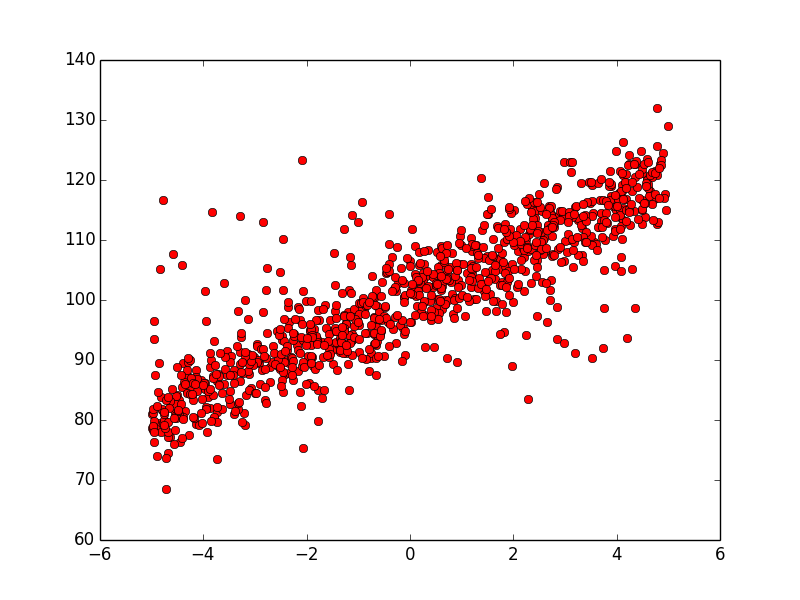
\includegraphics[width=100mm]{pics/graphic.png}
    \caption{Вывод графика рассеяния $(y_i,x_i)$\label{overflow}}
\end{figure}
\newpage

\section{Построение оценки параметров регресии с помощью группирования выборки}\label{sec4}
Будем работать с моделью регрессии (\ref{eq3}), предполагая что имеем регрессию без выбросов (\ref{eq1}). 
Каждый $y_i$ принадлежит нормальному распределению:
\begin{eqnarray}
    \label{eq12}y_i=f(x_i,\beta)+\varepsilon_i \sim \mathcal{N}(f(x_i,\beta),\sigma^2).
\end{eqnarray}
Разделим множество значений функции регрессии, т.е множество $\mathcal{R}$, на $k$ полуинтервалов:
\begin{eqnarray}
    \mathcal{R}=(-\infty,a_1]\bigcup(a_1,a_2]\bigcup \dots \bigcup(a_{k-1},+\infty ).
\end{eqnarray}
Обозначим полученные интервалы: $\nu_0,\dots,\nu_{k-1}$.\hfill\break
Далее в работе будем считать, что вместо истинных значений зависимых переменных $y_i$ наблюдается только номер класса, к которому это наблюдение попало.
Тогда для каждого $y_i$ будем набюдаем лишь номер полуинтервала $\mu_i$, в который он попал.
\begin{eqnarray}
    \mu_i=j, \textup{если $y_i$ отнесли к полуинтервалу $\nu_j$}.
\end{eqnarray}
Функцию распределения нормального закона с параметрами $\mu,\sigma^2$ можно представить как:
\begin{eqnarray}
    F(x)=\Phi(\frac{x-\mu}{\sigma}),
\end{eqnarray}
где $\Phi(x)$ функция распределения стандартного нормального закона, а $\sigma = \sqrt{\sigma^2}$:
\begin{eqnarray}
    \Phi(x)=\frac{1}{\sqrt{2}\sigma}\int_{-\infty}^{x}e^{\frac{-t^2}{2}}dt.
\end{eqnarray}
Обозначим:
\begin{eqnarray}
    \textup{erf}(x)=\frac{2}{\sqrt{\pi}}\int_0^{x}e^{-t^2}dt.
\end{eqnarray}
Тогда:
\begin{eqnarray}
    \Phi(x)= \frac{1}{2} \Big[1+\textup{erf}\Big(\frac{x}{\sqrt{2}} \Big) \Big].
\end{eqnarray}
Поэтому:
\begin{eqnarray}
    F(x)= \frac{1}{2} \Big[1+\textup{erf}\Big(\frac{x-\mu}{\sqrt{2}\sigma} \Big) \Big].
\end{eqnarray}
Тогда при модельных предположениях (\ref{eq12}) вероятность попадания $y_i$ в полуинтервал $\nu_j$ равна:
\begin{eqnarray}
    P\{y_i\in\nu_j\}= F_{y_i}(a_{j+1})-F_{y_i}(a_{j})=
\end{eqnarray}
\begin{eqnarray*}
    =
    \begin{cases}
        \frac{1}{2}(\textup{erf}(\frac{a_{j+1}-f(x_i,\beta)}{\sqrt{2}\sigma})-\textup{erf}(\frac{a_{j}-f(x_i,\beta)}{\sqrt{2}\sigma})),~j=\overline{1,k-2}\\
        \frac{1}{2}(1+\textup{erf}(\frac{a_{1}-f(x_i,\beta)}{\sqrt{2}\sigma})),~j=0\\
        \frac{1}{2}(1+\textup{erf}(\frac{a_{k-1}-f(x_i,\beta)}{\sqrt{2}\sigma})),~j=k-1
    \end{cases}.
\end{eqnarray*}
Понятно, что:
\begin{eqnarray}
    P(\mu_i=j)=P(y_i\in \nu_{\mu_i}).
\end{eqnarray}
\subsection{Построение функции правдоподобия}\label{sec4_1}
Составим функцию правдоподобия:
\begin{eqnarray}
    \label{eq22}l(\beta,\sigma^2, \nu_0,\dots, \nu_{k-1})=\textup{ln}(\prod_{i=1}^{n}P(\mu_i=j))=\\
    \label{eq23}=\sum_{i=1}^{n}\ln(P(\mu_i=j)).
\end{eqnarray}
Известно приближение для функции $\textup{erf}(x)$:
\begin{eqnarray}
    \label{eq24}(\textup{erf} x)^2\approx 1- \exp(-x^2 \frac{\frac{4}{\pi}+ax^2}{1+ax^2}),\\
    a=\frac{8}{3\pi}\frac{3-\pi}{\pi -4}.
\end{eqnarray}
Оно считается достаточно точным для $x$ близких к $0$ и к $\infty$ \cite{Winitzki}. \hfill\break
Найдем производную для этого приближения:
\begin{eqnarray}
    \label{eq26}\textup{erf}'(x) = \exp(-x^2 \frac{\frac{4}{\pi}+ax^2}{1+ax^2}) \frac{-2x\frac{\frac{4}{\pi}+ax^2}{1+ax^2}+(2ax^3)\frac{\frac{4}{\pi}+ax^2}{1+ax^2}-\frac{2ax^3}{1+ax^2}}{2\sqrt{1- \exp(-x^2 \frac{\frac{4}{\pi}+ax^2}{1+ax^2})}}.
\end{eqnarray}
Будем максимизировать функцию $l$.
Для этого будем искать нули ее производной. Вычисление будем производить с помощью вычислительных методов (будем использовать метод секущих), так как из-за сложного вида производной вычислить ее аналитически не представляется возможным.
\begin{eqnarray}
    \label{eq27}\frac{\delta l}{\delta \beta}=\frac{\delta \sum_{i=1}^{n}\ln(P(\mu_i=j))}{\delta \beta}=\frac{\delta \sum_{i=1}^{n}\ln P(y_i\in \nu_{\mu_i})}{\delta \beta}=~~~~~\\
    =\frac{\delta \sum_{i=1}^{n} \ln(\frac{1}{2}(\textup{erf}(\frac{a_{\mu_i+1}-f(x_i,\beta)}{\sqrt{2}\sigma})-\textup{erf}(\frac{a_{\mu_i}-f(x_i,\beta)}{\sqrt{2}\sigma})) )         }{\delta \beta}=~~~~~\\
    =  \sum_{i=1}^{n}\Big((1-(\delta_{\mu_i 0}+\delta_{\mu_i k-1}))\frac{(\textup{erf'}(\frac{a_{\mu_i+1}-f(x_i,\beta)}{\sqrt{2}\sigma})-\textup{erf'}(\frac{a_{\mu_i}-f(x_i,\beta)}{\sqrt{2}\sigma}))}{ (\textup{erf}(\frac{a_{\mu_i+1}-f(x_i,\beta)}{\sqrt{2}\sigma})-\textup{erf}(\frac{a_{\mu_i}-f(x_i,\beta)}{\sqrt{2}\sigma}))}+~~~~~\\
    \nonumber +(\delta_{\mu_i 0}+\delta_{\mu_i k-1})\frac{\textup{erf'}(\frac{a_{\mu_i}-f(x_i,\beta)}{\sqrt{2}\sigma})}{(1+\textup{erf}(\frac{a_{\mu_i}-f(x_i,\beta)}{\sqrt{2}\sigma}))}\Big)  (-1) \frac{\delta f(x_i,\beta)}{\delta \beta} )=~~~~~\\
    =-\sum_{i=1}^{n}\begin{pmatrix}
        1\\
        x_{i1}\\
        \dots\\
        x_{in}
    \end{pmatrix}\times  \Big((1-(\delta_{\mu_i 0}+\delta_{\mu_i k-1}))\frac{(\textup{erf'}(\frac{a_{\mu_i+1}-f(x_i,\beta)}{\sqrt{2}\sigma})-\textup{erf'}(\frac{a_{\mu_i}-f(x_i,\beta)}{\sqrt{2}\sigma}))}{ (\textup{erf}(\frac{a_{\mu_i+1}-f(x_i,\beta)}{\sqrt{2}\sigma})-\textup{erf}(\frac{a_{\mu_i}-f(x_i,\beta)}{\sqrt{2}\sigma}))}+~~~~~\\
    \nonumber +(\delta_{\mu_i 0}+\delta_{\mu_i k-1})\frac{\textup{erf'}(\frac{a_{\mu_i}-f(x_i,\beta)}{\sqrt{2}\sigma})}{(1+\textup{erf}(\frac{a_{\mu_i}-f(x_i,\beta)}{\sqrt{2}\sigma}))}\Big)  ,~~~~~
\end{eqnarray}
где $\delta_{ij}$ - символ Кронекера.\hfill\break
Доказано, что максимизируя функцию правдоподобия (\ref{eq22}), можем получить состоятельную оценку\cite{OLSforGrouping} параметров. \hfill\break
Итак, выражение (\ref{eq27}) и будем использовать для метода дихотомии, приближая $\textup{erf}'(x)$ с помощью выражения (\ref{eq26}).

\subsection{Метод секущих}\label{sec4_2}
Так как мы не можем привести систему $ \frac{\delta l}{\delta \beta}=0$ к виду, удобному для итерации, то нам придется искать ее нули с помощью метода Ньютона.
Введем вектор ошибки $\check{\varepsilon}^{(k)}=\beta^{*}-\beta^{(k)}$. Тогда для его определения имеем:
\begin{eqnarray}
    \frac{\delta l (\beta^{(k)}+\check{\varepsilon}^{(k)})}{\delta \beta}=0.
\end{eqnarray}
Строя разложение левой части по формуле Тейлора и ограничиваясь лишь линейными членами\cite{NumericalMethods}, будем иметь систему:
\begin{eqnarray}
    \frac{\delta }{\delta \beta}\frac{\delta l (\beta^{(k)}}{\delta \beta}\Delta \beta^{(k)}=-\frac{\delta l (\beta^{(k)})}{\delta \beta}.
\end{eqnarray}
Если матрица $\frac{\delta }{\delta \beta}\frac{\delta l (\beta^{(k)}}{\delta \beta}$ невырожденная (а в нашем случае она диагональная), то из этой системы можно единственным образом найти $\Delta \beta^{(k)}$ и построить приближение:
\begin{eqnarray}
    \beta^{(k+1)}=\beta^{(k)}+\Delta \beta^{(k)}.
\end{eqnarray}
Так как для второй производной $l$ получится довольно сложное выражение, то будем приближать ее с помощью выражения:
\begin{eqnarray}
    \frac{\delta }{\delta \beta_j}\frac{\delta l(\beta_1^{(k)},\dots, \beta_n^{(k)}) }{\delta \beta}\approx \frac{\frac{\delta l(\beta_1^{(k)},\dots,\beta_j^{(k)},\dots, \beta_n^{(k)}) (\beta^{(k)}}{\delta \beta}-\frac{\delta l(\beta_1^{(k)},\dots,\beta_j^{(k-1)},\dots, \beta_n^{(k)}) (\beta^{(k)}}{\delta \beta}}{\beta_j^{(k)}-\beta_j^{(k-1)}}.
\end{eqnarray}
Теперь имеем нули производной функции $l$, а также ее значения на границе отрезка $[a,b]$.
Переберем эти значения и таким образом найдем значение вектора $\hat{\beta}$, где она достигает своего максимального значения.
% \subsection{Оценка сходимости метода секущих}
% Так как метод секущих является частным случаем метода Ньютона, то приведем теоремы




\subsection{Переклассификация выборки}\label{sec4_3}
На данном этапе для каждого $x_i$ имеем класс $\mu_i$: т.е. пару $(x_i,\mu_i)$.
Теперь попытаемся переклассифицировать выборку. 
Для этом будем строить новую выборку такого же объема $N$.
Будем идти по каждому элементу $(x_i, \mu_i)$ выборки и для этого наблюдения построим новое:
\begin{equation}
    (x_i, \check{\mu}_i),
\end{equation}
где $\check{\mu}_i$ максимально встречающийся класс близлежайших $K$ соседей:
\begin{equation}
    \check{\mu}_i = \arg\max_j \sum_{x_j\in V_i,~j\neq i} \delta_{\check{\mu}_k j},
\end{equation}
где $(V_i)$ те $K$ наблюдений из $x_k, k=\overline{1,N}$, где .Чем он выше, тем больше используется соседей для коррекции класса нашего наблюдения.

Итак, переклассифицировав выборку, применим к ней функцию правдоподобия из уравнений (\ref{eq22}-\ref{eq23}), только используя теперь новые классы $\check{\mu}_i$ вместо $\mu_i$. 
Аналогично пунктам \ref{sec4_1}-\ref{sec4_2} максимизируем ее и найдем новую оценку параметров $\hat{\beta}$.

\newpage
\section{Реализация оценок на практике}
На практике построение оценок является нетривиальной задачей, так как метод секущих имеет свои недостатки.
Для метода секущих необходимо, чтобы корни уравнения были отделены, но не существует способа отделения корней в общем случае.
Поэтому для решения уравнения нам нужны дополнительные параметры:
\begin{itemize}
    \item границы отрезка, на котором находятся предполагаемая оценка $\hat{\beta}$,
    \item расстояние по норме между двумя начальными приближениями $\hat{\beta}^{(0)}, \hat{\beta}^{(1)}$,
    \item шаг для каждой переменной $\hat{\beta}_i^{(k)}$.
\end{itemize}
Тогда решая методом секущих уравнение
\begin{eqnarray}
    \frac{\delta l (\beta)}{\delta \beta}=0.
\end{eqnarray}
на каждом из отрезков найдем возможные $\hat{\beta}$. Найдя среди полученных приближений $\hat{\beta}$ то, 
на котором функция правдоподобия (\ref{eq22}-\ref{eq23}) достигает максимума, 
найдем решение.



\subsection{Эксперименты}
\begin{center}
    \begin{tabular}{|p{5cm}|p{5cm}|}
        \hline
        \multicolumn{2}{|c|}{Параметры программы} \\
        \hline
        Переменная&значение\\
        \hline
        Размер выборки $N$& 100\\
        \hline
        Доля выбросов $\widetilde{\varepsilon}$& 0.8\\
        \hline
        Параметры регрессии $\beta$& $(90,4)$\\
        \hline
        Регрессоры $x_i$ & $\sim U(-5,5)$\\
        \hline
        $\varepsilon_i$&$\sim N(0,16)$\\
        \hline
        $\eta_i$&$\sim N(100,100)$\\
        \hline
    \end{tabular},
    \end{center}
построим для начала 100 оценок $\hat{\beta}$ при разных выборках:

\newpage
\begin{figure}[ht!]
    \centering
    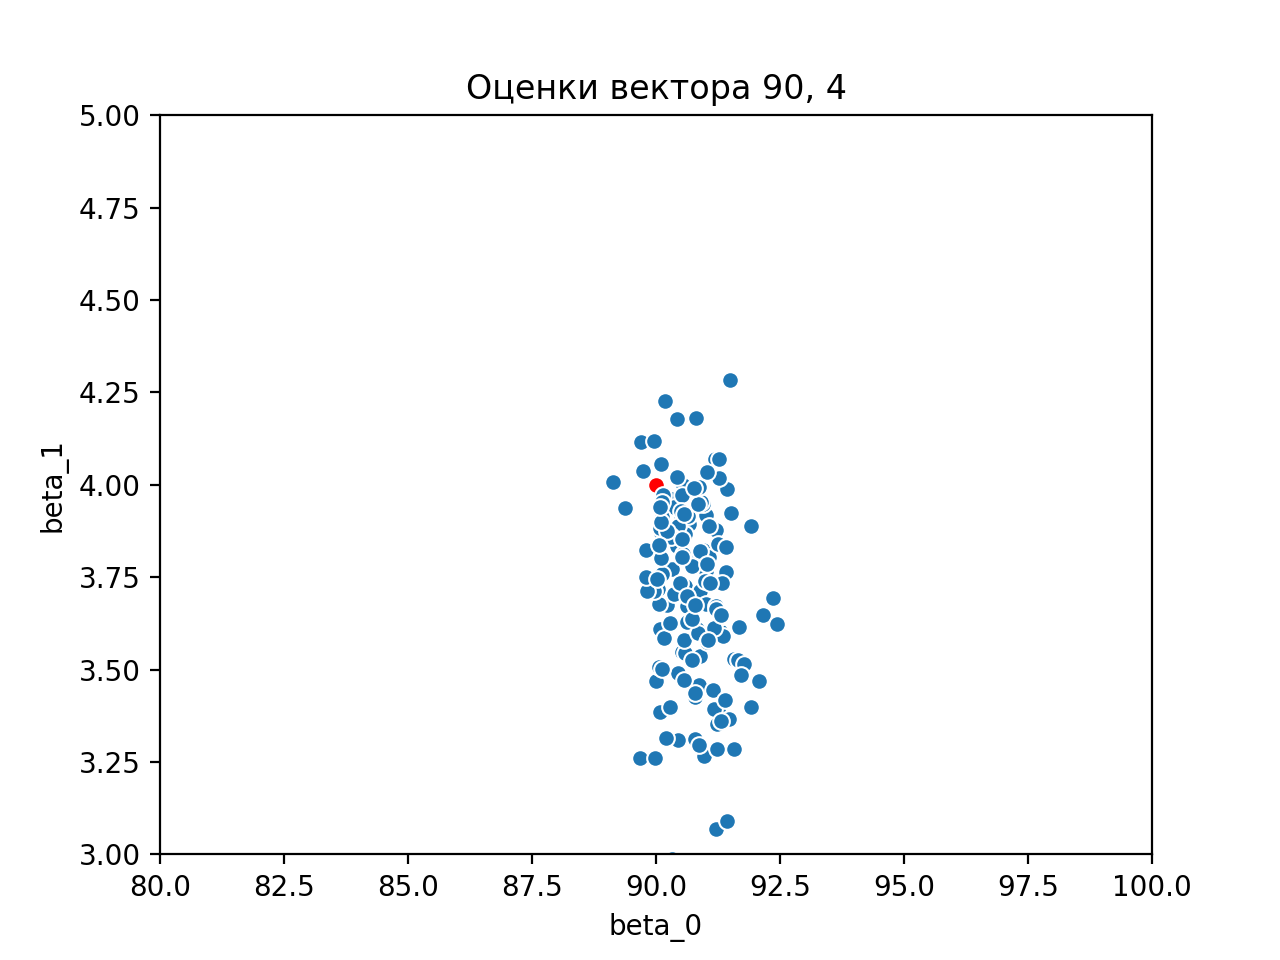
\includegraphics[width=100mm]{pics/plot_90_4_(2).png}
    \caption{Вывод графика рассеяния $(\hat{\beta}_0,\hat{\beta}_1)$ красным - истинное значение\label{overflow}}
\end{figure}

теперь  100 оценок $\hat{\beta}$ при выключенной классификации и выключенной:
\begin{figure}[h]
    \centering
    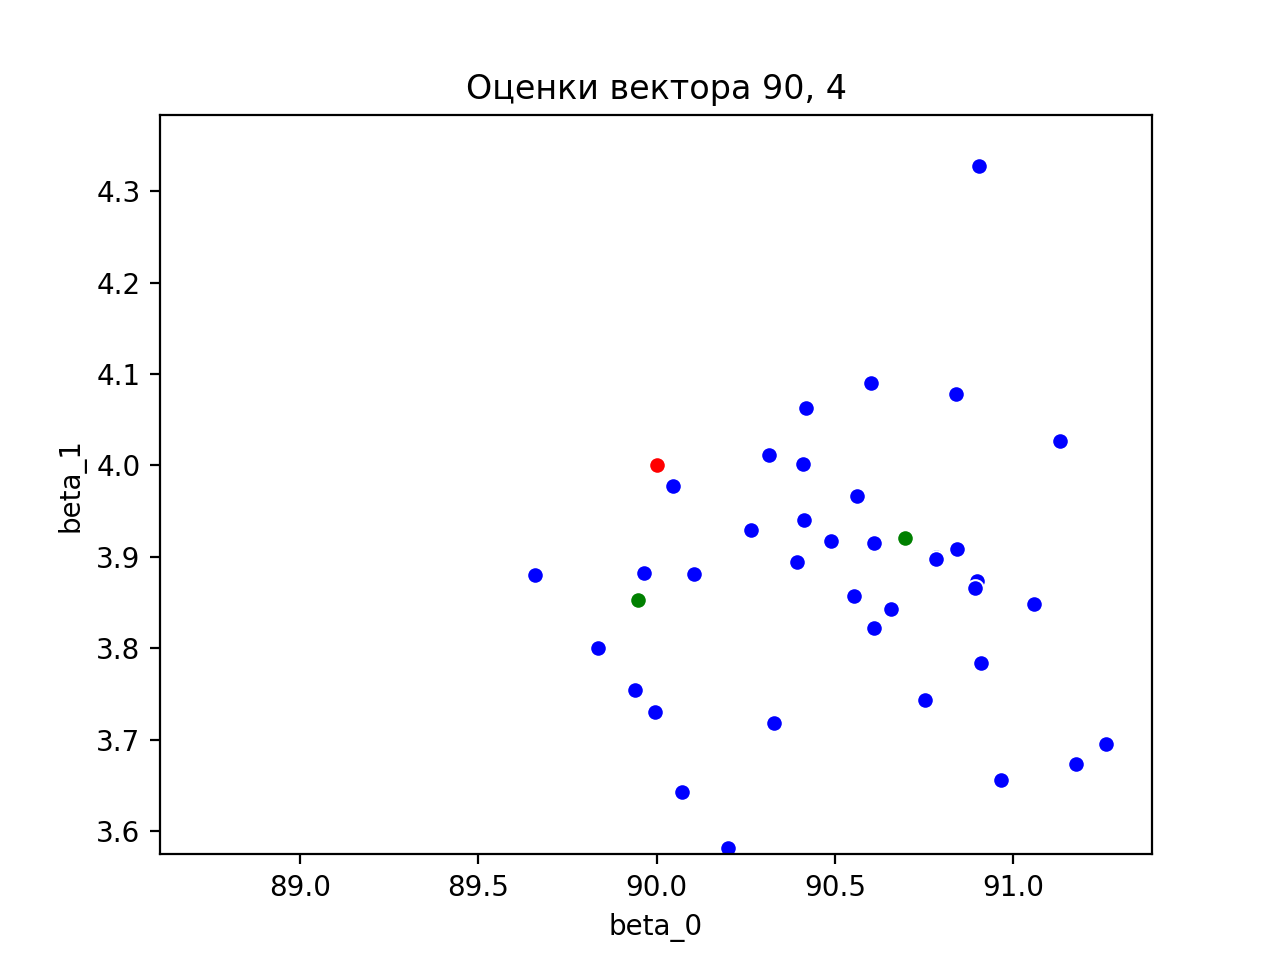
\includegraphics[width=100mm]{pics/plot_90_4_with-without_(2).png}
    \caption{Вывод графика рассеяния $(\hat{\beta}_0,\hat{\beta}_1)$\label{overflow}}
    \label{pic_3}
\end{figure}
\break
На графике \ref{pic_3} зеленым цветом обозначены приближения без классификации, синим с классификацией, а красным - истинное значение.
\newpage
\begin{figure}[ht]
    \centering
    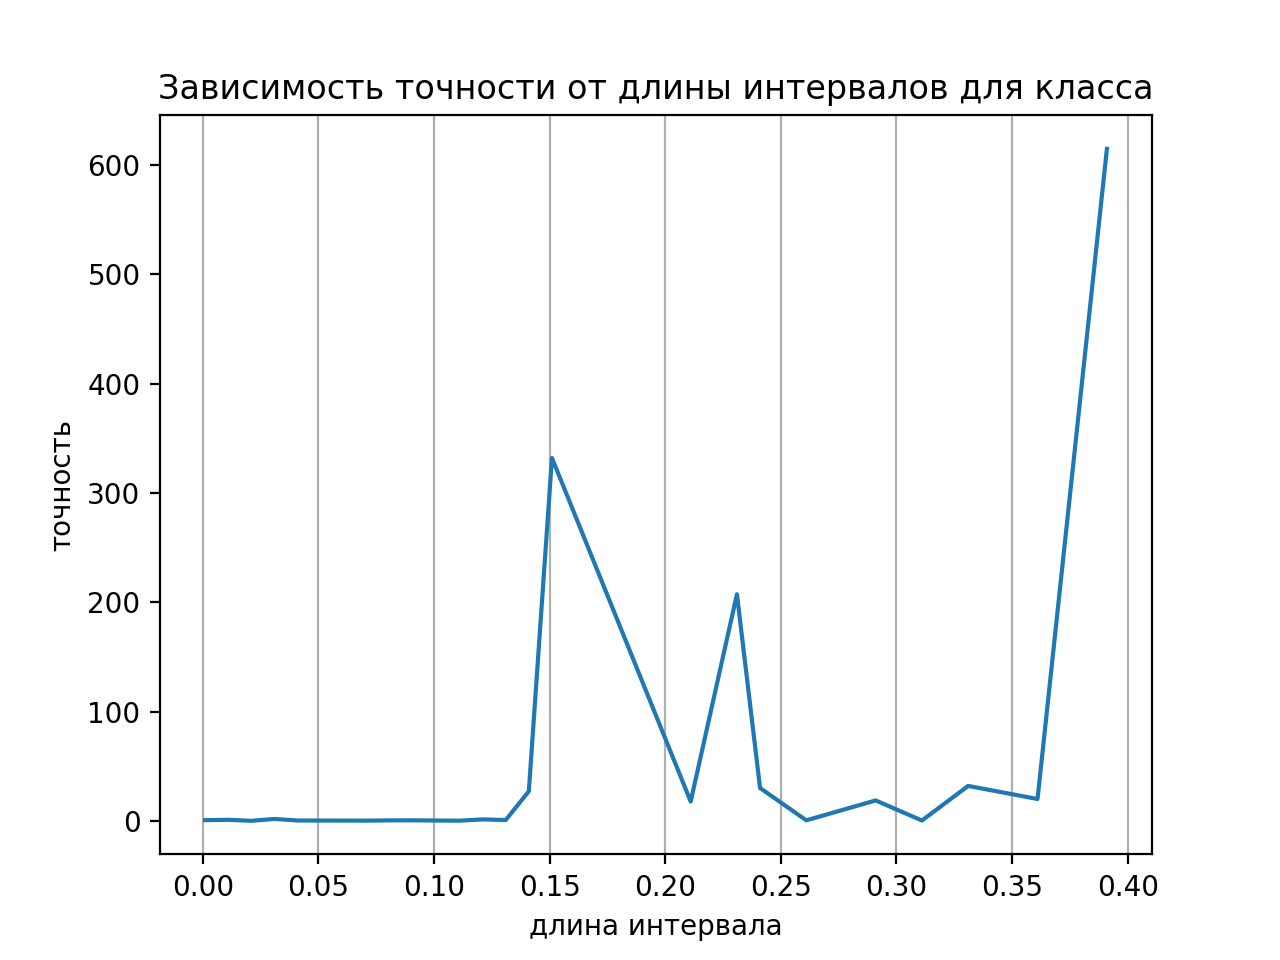
\includegraphics[width=100mm]{pics/plot_90_4_accuracy-length.png}
    \caption{Зависимость точности от длины интервала\label{overflow}}
    \label{pic_3}
\end{figure}
\begin{figure}[h]
    \centering
    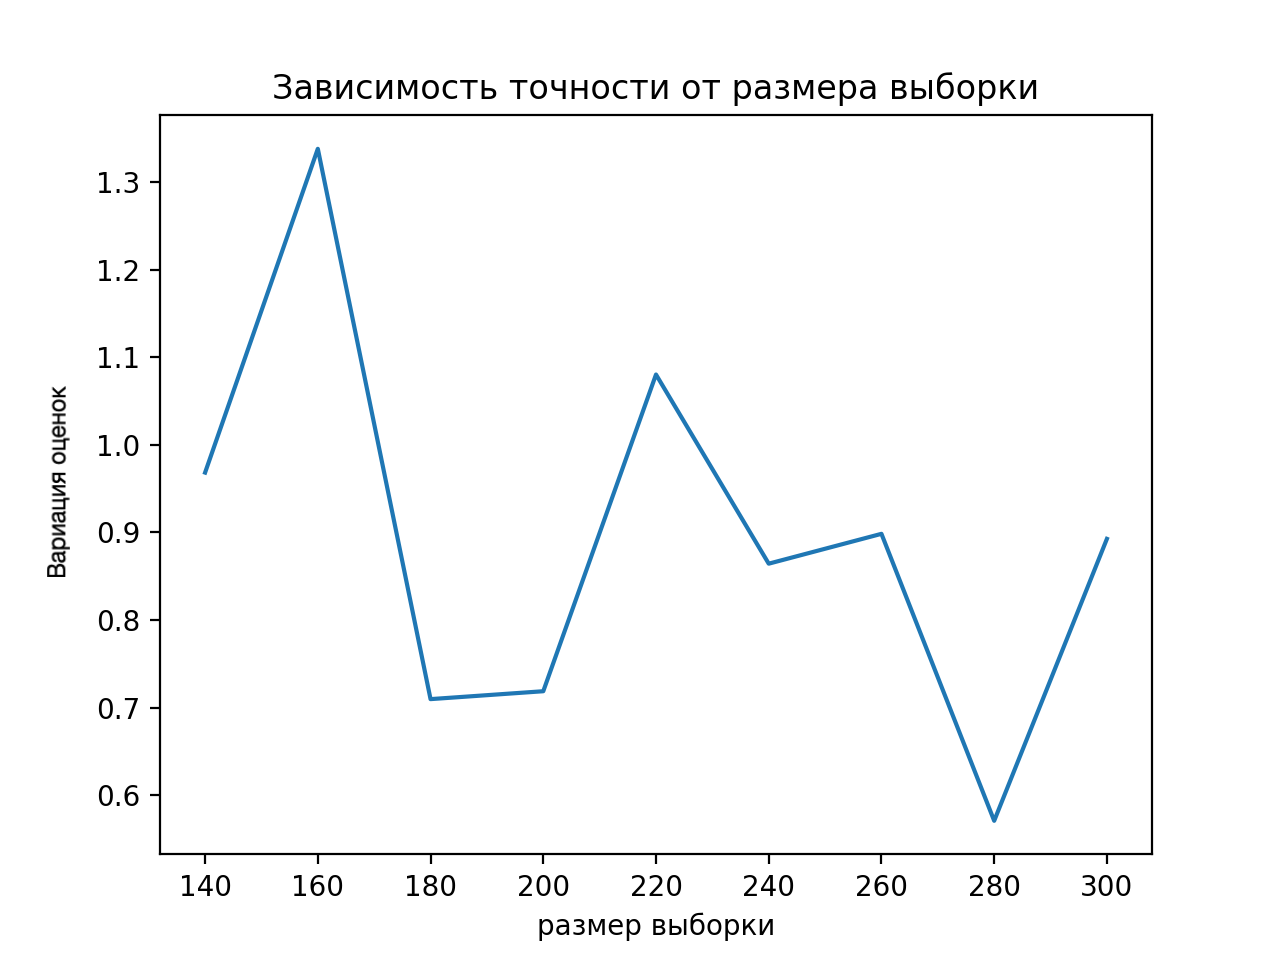
\includegraphics[width=100mm]{pics/plot_90_4_accuracy-samplesize.png}
    \caption{Зависимость точности от размера выборки\label{overflow}}
    \label{pic_3}
\end{figure}
Видим, что точность увеличивается при увеличении выборки и падает при уменьшении точности классифицирования. Метод в общем случае дает достаточно хорошее приближение к точному значению.
\newpage
\section{Приложение}
\section{Листинг некоторых методов}
Метод секущих:
\begin{verbatim}
def fit_intercept(self, beta_hat=None, beta_hat_next=None):
    if beta_hat is None:
        beta_hat = np.matrix(np.zeros(self.exogen[0].size)).T

    if beta_hat_next is None:
        beta_hat_next = np.matrix(np.ones(self.exogen[0].size)).T

    iteration_counter = 0
    while np.linalg.norm(beta_hat - beta_hat_next) > Defines.METHOD_ACCURACY:
        if self._shared_stop_event.is_set():
            raise StopIteration("fit: got stop event")
        if iteration_counter < Defines.COUNT_LIMIT_OPERATIONS:
            iteration_counter += 1
            dlikelihood_f_for_beta_hat_next = self.full_cl_recl_dlikelihood_f(beta_hat_next)
            delta_beta = np.matrix(np.zeros(self.exogen[0].size)).T

            dlikelihood_derivative_approximation = np.zeros((self.exogen[0].size,
             self.exogen[0].size))

            for i in range(self.exogen[0].size):
                temp_beta = copy.deepcopy(beta_hat_next)
                temp_beta[i] = beta_hat[i]
                dlikelihood_derivative_approximation[i] = ((self.full_cl_recl_dlikelihood_f(
                    beta_hat_next) - self.full_cl_recl_dlikelihood_f(temp_beta)) 
                            / (beta_hat_next[i] - beta_hat[i])).A1

            delta_beta = (- np.matrix(dlikelihood_f_for_beta_hat_next)[0] * np.linalg.inv(
                dlikelihood_derivative_approximation))
            beta_hat = beta_hat_next
            beta_hat_next = beta_hat_next + delta_beta.T
        else:
            raise StopIteration("fit: fit_intercept has achieved iteration limit")

    return beta_hat_next
\end{verbatim}
Решение методом секущих:
\begin{verbatim}
def fit(self):
    print("")
    self.classify()
    self.reclassify(Defines.RECLASSIFICATION_LEVEL)

    print("fit: fitting.....")

    t_beta_hat = np.matrix([80.0, 0.0]).T
    t_beta_hat_next = np.matrix([100.0, 10.0]).T
    right_bound_indent = Defines.right_bound_fit_indent(self.exogen[0].size)
    loop_indentantion_value = Defines.LEFT_BOUND_EVERY_VAR_INDENT
    loop_end_bound = Defines.fit_loop_stop_value(self.exogen[0].size)

    beta_hats_left_bound = Defines.left_bound_fit_init(self.exogen[0].size)

    def recursive_beta_generator(index, previous_step_beta):
        assert (index <= self.exogen[0].size)

        beta_next = np.matrix.copy(previous_step_beta)

        while ((beta_next + right_bound_indent) < loop_end_bound).all():
            if index == self.exogen[0].size:
                yield beta_next
                break

            beta_next[index] += loop_indentantion_value

            next_index_generator = recursive_beta_generator(index + 1, beta_next)
            for item in next_index_generator:
                yield item

    fit_intercept_results = []

    def fit_intercept_and_add_to_results(beta_hat_one, beta_hat_two):
        t_result = self.fit_intercept(beta_hat_one, beta_hat_two)
        if (np.isnan(t_result) == False).all():
            print("fit: added value to list %s" % t_result)
            fit_intercept_results.append(t_result)
        else:
            raise Exception("fit: got nan")

    created_threads = []
    for beta_left in recursive_beta_generator(0, beta_hats_left_bound):
        beta_right = beta_left + right_bound_indent
        calculus_thread = Thread(target=fit_intercept_and_add_to_results, args=(np.matrix.copy(beta_left),
                                                                                np.matrix.copy(
                                                                                    beta_right)))
        created_threads.append(calculus_thread)
        calculus_thread.start()

    for thread in created_threads:
        thread.join(timeout=Defines.THREAD_JOIN_TIMEOUT)

    maximum_likelihood_res = None
    result_to_return = np.matrix([None for _ in range(self.exogen[0].size)]).T

    print("fit: possible betas: ")
    print(fit_intercept_results)

    initial_left_bound = Defines.left_bound_fit_init(self.exogen[0].size)
    initial_right_bound = loop_end_bound

    self._shared_stop_event.set()

    for result in fit_intercept_results:
        if (result < initial_left_bound).any():
            continue

        if (result > initial_right_bound).any():
            continue

        t_likelihood_res = self.full_cl_recl_likelihood_f(result)
        # print(t_likelihood_res)
        if maximum_likelihood_res is None:
            maximum_likelihood_res = t_likelihood_res
            result_to_return = result

        if maximum_likelihood_res < t_likelihood_res:
            maximum_likelihood_res = t_likelihood_res
            result_to_return = result

    return result_to_return
\end{verbatim}
\newpage
\section{Заключение}
Были описаны некоторые методы робастного оценивания параметров регрессии.
Был предложен еще один способ оценивания параметров регрессии для модели регрессии с аномальными наблюдениями при наличии группирования выборки. 
Оценки из пункта \ref{sec4} были реализованы на практике. Построенный метод был исследован на точность.
\newpage
% \section{Список литературы}
% \printbibliography
\begin{thebibliography}{8}
    \bibitem{Huber}
    Хьюбер Дж П.,
    \textit{Робастность в статистике:пер. с англ.}.
    М.:Мир,1984-304с

    \bibitem{OLSforGrouping}
    Е. С Агеева, чл.-корр. НАН Беларуси Ю.С. Харин,
    \textit{Состоятельность оценки максимального правдопобия параметров множественной регрессии по классифицированным наблюдениям}

    \bibitem{Kharin}
    Харин Ю.С., Зуев Н.М.,
    Жук Е.Е,
    \textit{Теория вероятностей, математическая и прикладная статистика: учебник}
    Минск: БГУ, 2011.-463с

    \bibitem{RobustRegression}
    John Fox \& Sanford Weisberg,
    \textit{Robust Regression},
    October 8, 2013

    \bibitem{RobustPolynomialEstimation}
    А.В. Омельченко,
    \textit{Робастное оценивание параметров полиномиальной регрессии второго порядка,}
    Харьковский национальный университет радиоэлектроники, Украина, 2009

    \bibitem{ComparisonRobust}
    \"{O}zlem G\"{u}r\"{u}nl\"{u} Alma,
    \textit{Comparison of Robust Regression Methods
    in Linear Regression},
    Int. J. Contemp. Math. Sciences, Vol. 6, 2011, no. 9, 409 - 421

    \bibitem{Winitzki}
    Sergei Winitzki,
    \textit{A handy approximation for the error function and its inverse}

    \bibitem{NumericalMethods}
    Мандрик П.А., Репников В.И., Фалейчик Б.В.,
    \textit{Численные методы}
\end{thebibliography}
\addcontentsline{toc}{section}{Список Литературы}
\end{document}